\section*{Problem 2}

\begin{figure}[H]
\caption*{}
\centering
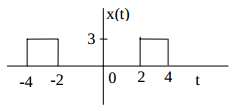
\includegraphics[width=0.4\textwidth]{figs/c2p2.png}
\label{fig:c2p2}
\end{figure} 

\subsection*{Solution}

Lets call $x_{p1}(t)$ and $X_{p1}(\omega)$ the function in time domain of the first point 
and its Fourier Transform respecively. 
We can express our function in terms of such function as:

\begin{equation*}
x(t) = \frac{3}{2} [x_{p1}(t-2) + x_{p1}(t+4)]
\end{equation*} 

As we can see from (\ref{eq:c22b}) the displacement in time is reflected in the
frecuency domain as a multiplication by an exponential. 

\begin{equation*}
\begin{aligned}
X(\omega) &= \frac{3}{2} X_{p1}(\omega) [ e^{- 2 j \omega} + e^{4 j \omega} ] \\
&= \frac{3}{2} X_{p1}(\omega) e^{j \omega} [ e^{- 3 j \omega} + e^{3 j \omega} ] \\
&= 12 Sa(\omega) \cos(3 \omega)
\end{aligned}
\end{equation*} 

The plot of the magintude and angle of $X(\omega)$ is:
\zcodemat{sources/c2p2a.m}{Plot of Magnitude and Angle}

\begin{figure}[H]
\caption{Magnitude $|X(\omega)|$ and Angle}
\centering
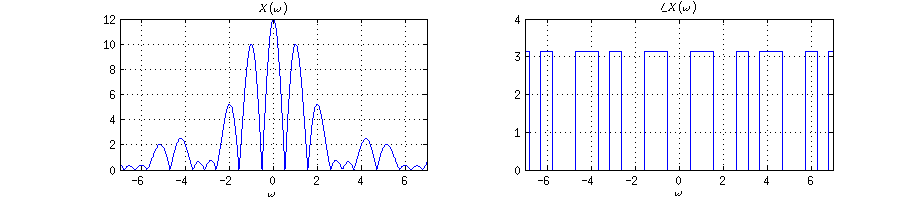
\includegraphics[width=1.0\textwidth]{figs/c2p2a.png}
\label{fig:c2p2a}
\end{figure} 

